\section{Pubblicità}

Le pubblicità sono state assenti dal dominio per molti anni: infatti è un servizio gratuito
offerto da volontari. Sono state introdotte solo qualche mese addietro, per poter compensare
almeno parzialmente ai costi dei server.

\subsection{Posizionamento}
Le pubblicità, per essere visualizzate il più possibile, devono essere piazzate nelle zone del
layout che vengono viste maggiormente dall'utente. Nel sito, le pubblicità sono posizionate
come nell'immagine a seguire (come era visibile anche nella figura \ref{homepage}).

\begin{figure}[hbt]
    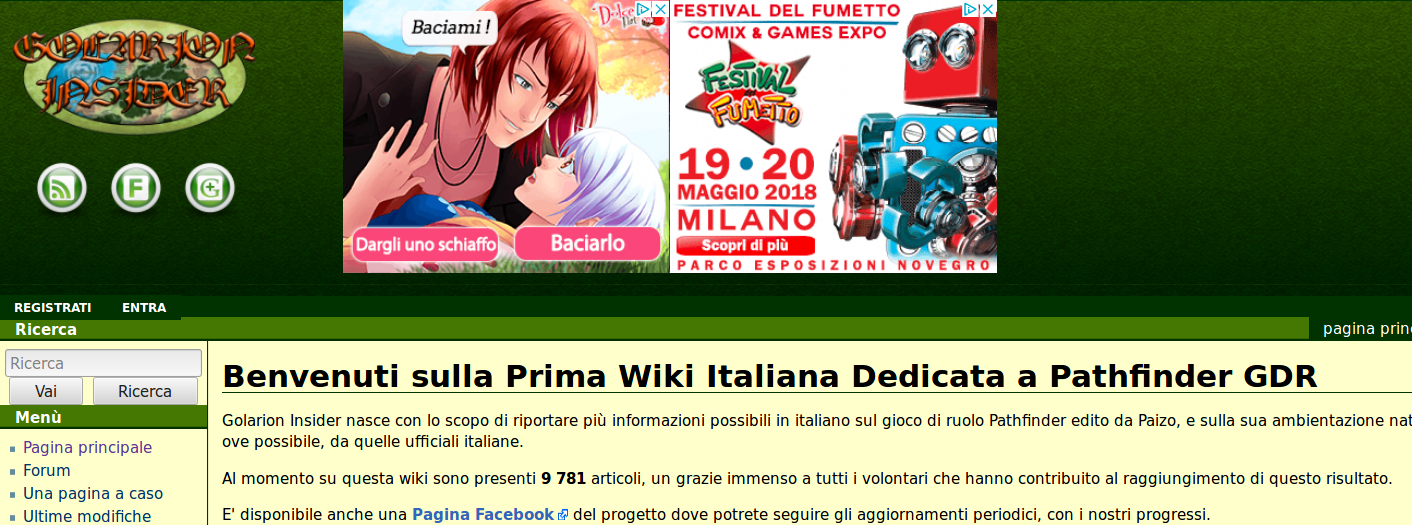
\includegraphics[width=\textwidth]{img/pubblicita.png}
    \caption{La pubblicità, \href{http://golarion.altervista.org/wiki/Pagina_principale}{Homepage - Golarion Insider}}
\end{figure}

Essendo un banner presente nell'\emph{header}, affianco al logo, la pubblicità difficilmente non verrà vista 
dal visitatore. Questa è una buona scelta per il posizionamento.\par
Ciò che non va bene, è il tipo di pubblicità. Esse non rispecchiano minimamente le preferenze degli utenti, 
sono casuali e potrebbero infastidire chi ha meno pazienza.
Fortunatamente, non sono presenti altre forme di pubblicità (pop-up, video che partono in \emph{autoplay}, etc\dots),
ed è l'unico banner presente nell'intera pagina. In questo modo, l'usabilità non è compromessa in alcun modo.